%!TEX root = TQFTbook.tex
%%%%%%%%%%%%%%%%%%%%%%%%%%%%%%
\chapter{Extended 2d TQFT}\label{c:2d-extended}

In this chapter we define the notion of extended 2d TQFT and classify such
TQFTs. Our exposition is based on Schommer-Pries' thesis \cite{schommer-pries}.


Informally, an extended 2d TQFT is a theory in which we allow:
\begin{itemize}
  \item 0-dimensional manifolds
  \item 1-dimensional cobordisms between 0d manifolds
  \item 2-dimensional cobordisms between them
\end{itemize}
and to each of those, assign corresponding algebraic data (to be
specified later), subject to appropriate gluing laws.

As mentioned before, the natural language for this is the language of (weak)
2-categories: the 0-, 1-, and 2-dimensional manifolds and bordisms form a
2-category, which we will denote by $\Bord_2$; this category has a natural
symmetric monoidal structure, given by disjoint union. Thus, we give the
following preliminary definition.

\begin{predefinition}
  An extended 2d TQFT is a functor of symmetric monoidal 2-categories
  $$
    Z\colon \Bord_2\to \calC
  $$
  where $\calC$ is a target symmetric monoidal 2-category.
\end{predefinition}
Note that unlike the unextended case, where there is a standard choice of
the target category $\calC$ (namely, the category $\vect$), in the extended case
the choice of $\calC$ is less clear. We will discuss it later.

To make this definition precise, we need to actually define the
2-category $\Bord_2$.

%%%%%%%%%%%%%%
\section{Defining $\Bord_2$}\label{s:defining-bord2}
We begin with defining manifolds with corners. Note that there are two
approaches to defining manifolds: one can either use coordinate charts and
atlases, or sheaves of smooth functions. We will use the second approach.

For a topological space $X$, denote by $\mathscr{C}_X$ the sheaf of continuous
functions on $X$.%FIXME


\begin{definition}\label{d:manifold-corners}\index{manifold!with corners}
  An $n$-dimensional manifold with corners is a topological space $M$ with a
  subsheaf $\calF\subset \mathscr{C}_M$ such that for each point $x\in M$ there
  exists a homeomorphism of a neighborhood of $x$ in $M$ and a neighborhood of
  $0$ in
  $$
    \R_+^p\times \R^{n-p}
  $$
  which identifies the sheaf $\calF$ with the sheaf of smooth functions
  on $\R_+^p\times \R^{n-p}$ (we call a function on $\R_+^p\times
  \R^{n-p}$ smooth if it is a restriction of a
  smooth function on $\R^n$).
\end{definition}
It is easy to show that the number $p$ is well-defined: for different $p$,
the sets $\R_+^p\times \R^{n-p}$ are not diffeomorphic. We will call this
number the index of $x$; the set
$$
  \del^{(p)}(M)=\{x\st \text{index}(x)=p\}
$$
is the codimension-$p$ stratum of the boundary. In particular, we will call
connected components of $\del^{(1)}M$ \emph{faces}.

For technical reasons, we will impose an additional requirement that each point
$x\in M$ of index $p$ lies in the closure of exactly $p$ \textbf{different} faces;
thus,
we do not allow a face to ``intersect itself''. Following
\cite{schommer-pries}, we call such a manifold ``manifold with faces''.

Using this, we can give a definition of a 2-cobordism.

\begin{definition}\label{d:2-cobordism}\index{2-cobordism}
  Let $Y_0, Y_1$ be closed $(n-2)$-dimensional manifolds, and let
  $W_0,W_1$ be two $(n-1)$-dimensional cobordisms between $Y_0$ and $Y_1$.
  A 2-cobordism from $W_0$ to $W_1$ is the following collection of
  data:
  \begin{itemize}
    \item An $n$-dimensional manifold $S$ with corners of codimension up to 2.
    \item A decomposition of the set of faces of $S$ into two disjoint sets,
      ``horizontal faces'' and ``vertical faces'', such that each
      $x\in \del^{(2)}S$
      is in the closure of one vertical and one horizontal face. We will
      denote by $\del_h S$ the union of closures of horizontal faces,
      and similarly for vertical faces.
    \item An isomorphism $g\colon \ov{W_0}\sqcup W_1\to \del_h S$.
    \item An isomorphism $f\colon (Y_0\times I) \sqcup (Y_1\times I)\to \del_v S$.
  \end{itemize}
  These isomorphisms must agree with the isomorphisms
  $\ov{Y_0}\sqcup Y_1\isoto \del W_i$ in the obvious way.
\end{definition}
%% definition of 2-category of bordisms
\begin{center}
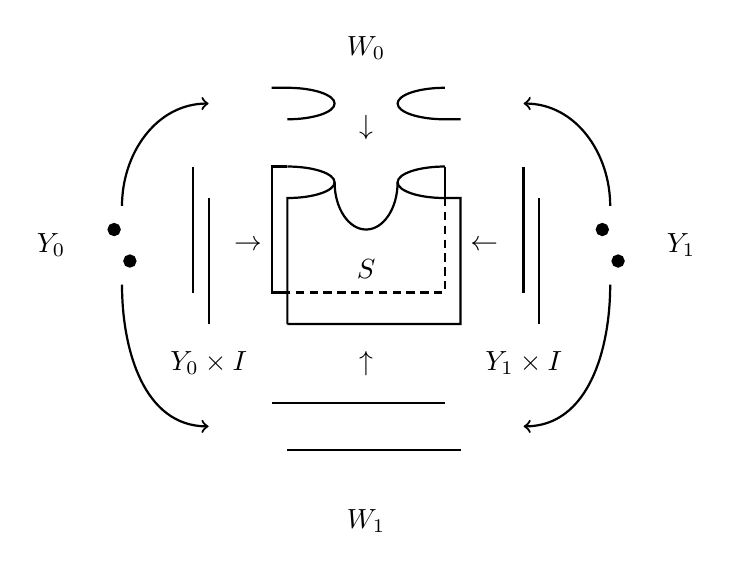
\begin{tikzpicture}[thick, scale = 2]
  % top
  \draw (1, 3.5) arc (90: 270: 0.3cm and 0.1cm) -- (1.1, 3.3) ;
  \draw (-.1, 3.5) -- (0,3.5) arc (90: -90: 0.3cm and 0.1cm);
  \node at (0.5, 3.75) {$W_0$};
  \node at (0.5, 3.25) {$\downarrow$};


  % main
  \draw (0, 3) arc (90: -90: 0.3cm and 0.1cm) -- (0, 2);
  \draw (1, 3) arc (90: 270: 0.3cm and 0.1cm) -- (1.1, 2.8) -- (1.1, 2) -- (0,
  2);
  \draw (1,3) -- (1, 2.8); \draw [densely dashed] (1, 2.8) -- (1, 2.2) --
  (0,2.2);
  \draw (.3, 2.9) arc (180: 360: 0.2cm and 0.3cm);
  \draw (0, 3) -- (-.1, 3) -- (-.1, 2.2) -- (0, 2.2);
  \node at (0.5, 2.35) {$S$};

  % bottom
  \draw (-0.1, 1.5) -- (1,1.5) (0,1.2) -- (1.1, 1.2);
  \node at (0.5, 0.75) {$W_1$};
  \node at (0.5, 1.75) {$\uparrow$};

  % left
  \draw (-0.5, 2.8) -- (-0.5, 2) (-0.6, 3) -- (-0.6, 2.2);
  \filldraw (-1, 2.4) circle (1pt) (-1.1, 2.6) circle (1pt);
  \node at (-1.5, 2.5) {$Y_0$};
  \node at (-0.5,1.75) {$Y_0 \times I$};
  \node at (-0.25, 2.5) {$\rightarrow$};
  \draw [->] (-1.05, 2.75) to [out=90, in = 180] (-0.5, 3.4);
  \draw [->] (-1.05, 2.25) to [out=270, in = 180] (-0.5, 1.35);

  % right
  \draw (1.6, 2.8) -- (1.6, 2) (1.5, 3) -- (1.5, 2.2);
  \filldraw (2.1, 2.4) circle (1pt) (2, 2.6) circle (1pt);
  \node at (2.5, 2.5) {$Y_1$};
  \node at (1.5,1.75) {$Y_1 \times I$};
  \node at (1.25, 2.5) {$\leftarrow$};
  \draw [->] (2.05, 2.75) to [out=90, in=0] (1.5,3.4);
  \draw [->] (2.05, 2.25) to [out=270, in=0] (1.5,1.35);
\end{tikzpicture}
\end{center}

We define an isomorphism of two 2-cobordisms $(S, g,f)$, $(\tilde S, \tilde
g, \tilde f)$ (for the same $Y_0,Y_1, W_0, W_1$) as a diffeomorphism $\ph\colon
S\to \tilde S$ such that $\ph\circ g = \tilde g$, $\ph\circ f=\tilde f$.

We can now give a definition of the 2-category $\Bord_2$.

\begin{theorem}\label{t:bord2}
  There exists a weak 2-category $\Bord_2$, in which
  \begin{itemize}
    \item Objects are closed oriented $0$-manifolds
    \item 1-morphisms $\Hom(X_0, X_1)$ are oriented 1-dimensional cobordisms
      between $X_0, X_1$
    \item For $W_0, W_1\in \Hom(X_0, X_1)$, the set of 2-morphisms
       $\Hom(W_0,W_1)$ is the set of isomorphism classes of 2-cobordisms
       $W_0\cob{}W_1$
  \end{itemize}
\end{theorem}
To prove this theorem, one has to construct horizontal and vertical
compositions, and prove strict associativity of vertical composition and
weak associativity of horizontal composition. Vertical composition is
relatively straightforward; it is done in the same way as the usual
composition of cobordisms.

However, horizontal composition is much trickier. Recall that for two
1-cobordisms $W_1$, $W_0$, the smooth structure on the glued 1-manifold
$W_0\cup_{Y_1} W_1$ is not unique. It was not a problem for a 1-d TQFT, where
1-morphisms are isomorphism classes of cobordisms; however, to define extended
2d TQFT, we need to define 2-cobordism between 1-morphisms, and for that we
need actual 1-cobordisms, not isomorphism classes.

There are two ways to deal with it. One can just randomly choose a smooth
structure on any result of gluing $W_0\cup_{Y_1} W_1$, using the axiom of choice;
this makes composition not strictly associative but only associative up to
isomorphism of 1-cobordisms (as is expected in a weak 2-category), but luckily
creates no other issues. The other, less arbitrary, approach is to add more
structure to 1-cobordisms --- collars or a similar data; in
\cite{schommer-pries}, he uses a structure he calls ``halo''. Both of these
approaches give a weak 2-category, and in fact they give equivalent
2-categories, see \cite[Proposition 3.40]{schommer-pries}.

We do not give details of either of these constructions, referring the reader to
\cite{schommer-pries}; this takes a significant part of his thesis.


\begin{theorem}\label{t:bord2-monoidal}
  The 2-category $\Bord_2$ defined in \thref{t:bord2} has a natural
  structure of a symmetric monoidal 2-category, with tensor product given
  by disjoint union.
\end{theorem}
This seems obvious, but remarkably, requires some machinery to do carefully.
See \cite{shulman}, \cite[Section 3.1.4]{schommer-pries}.

%%%%%%%%%%%%%%
\section{Definition of 2d extended TQFT}\label{s:def-2d-extended-tqft}
Now that we have defined the 2-category of bordisms, we can give a definition
of an extended 2d TQFT.



\begin{definition}\label{d:2d-etqft}\index{TQFT!extended 2d}
  Let $\calC$ be a symmetric monoidal 2-category. A $\calC$-valued
  extended 2d TQFT is a symmetric monoidal functor
  \begin{equation}\label{e:etqft-def}
    Z\colon \Bord_2\to \calC.
  \end{equation}
\end{definition}

Note that this is only one of several approaches to extended field theories. It
has some limitations: for example, by definition, in a 2-category we only have
2-morphisms $\al\colon f\to g$ if $f,g$ are 1-morphisms between the same
objects. For instance, the 2-dimensional manifold with corners shown below
cannot be considered a 2-cobordism:
$$
  \begin{tikzpicture}[scale=0.7]
    \draw[lightyellow] (-0.5,0) to[out = -90, in =90] (-1.5,-2)
          -- (-0.5,-2) to[out = 90, in =90, looseness = 2] (0.5,-2)
          -- (1.5, -2) to[out =90, in =-90] (0.5, 0)--cycle;
    \draw[thick, ->] (-0.5,0) -- (0.5,0);
    \draw[thick, ->](-1.5,-2) -- (-0.5,-2);
    \draw[thick, ->](0.5,-2) -- (1.5,-2);
  \end{tikzpicture}
$$

There are alternative approaches; for $n=2$, there is a notion of
``open-closed'' TQFT, studied in \cite{lauda-pfeiffer}, which allows
2-manifolds with corners similar to the one shown above.
Yet one more approach is the notion of ``TQFT with defects'', as discussed,
e.g., in \cite{dkr}, \cite{carqueville}. We will talk about these
approaches later.

%%%%%%%%%%%%%%
\section{Generators and relations of $\Bord_2$}\label{s:bord2-generators-relations}
%% \begin{figure}[ht]
% %  %\begin{center}
% %  \begin{tikzpicture}
% %    \node at (-6, 1.5) {\small Generating Objects:};
% %    % objects:
% %    \node at (-4, 1.5) {\footnotesize + {\tiny $\bullet$}};
% %    \node at (-3, 1.5) {- {\tiny $\bullet$}};
% %    \node at (0, 1.5) {\small Generating 1-Morphisms:};
% %    % 1-morphisms
% %    \begin{scope}[xshift = 9cm, yshift = 2.1 cm]
% %      \draw (-6.6, -.5) -- (-6.5, -.5) arc (90: -90: 0.3cm and 0.1cm);
% %      \draw (-5.5, -.5) arc (90: 270: 0.3cm and 0.1cm) -- (-5.4, -.7);
% %      \node at (-6.8, -.5) {\tiny +};
% %      \node at (-6.7, -.7) {-};
% %      \node at (-5.3, -.5) {\tiny +};
% %      \node at (-5.2, -.7) {-};
% %    \end{scope}
% %  \end{tikzpicture}
% %
% %  \begin{tikzpicture}
% %    \node at (-6, .5)   {\small Generating};
% %    \node at (-6, 0)   {\small 2-Morphisms:};
% %    \node at (-1,0) {
% %      $ \underbrace{
% %        \begin{tikzpicture}
% %          % Draw the saddle, curve up
% %          \draw (0, 3) arc (90: -90: 0.3cm and 0.1cm) -- (0, 2);
% %          \draw (1, 3) arc (90: 270: 0.3cm and 0.1cm) -- (1.1, 2.8) -- (1.1,
% %2) -- (0, 2);
% %          \draw (1,3) -- (1, 2.8); \draw [densely dashed] (1, 2.8) -- (1, 2.2)
% %-- (0,2.2);
% %          \draw (.3, 2.9) arc (180: 360: 0.2cm and 0.3cm);
% %          \draw (0, 3) -- (-.1, 3) -- (-.1, 2.2) -- (0, 2.2);
% %          % Draw saddle, curve down
% %          \draw (2,2) arc (-90: 0: 0.3cm and 0.1cm);
% %          \draw [densely dashed] (2.3, 2.1) arc (0:90: 0.3cm and 0.1cm);
% %          \draw (2, 2.2) -- (1.9, 2.2) -- (1.9, 3) -- (3,3) -- (3, 2.8);
% %          \draw [densely dashed] (3, 2.8) -- (3, 2.2);
% %          \draw (2,2) -- (2, 2.8) -- (3.1, 2.8) -- (3.1, 2) -- (3,2);
% %          \draw (3,2) arc (270: 180: 0.3cm and 0.1cm);
% %          \draw [densely dashed] (3, 2.2) arc (90: 180: 0.3cm and 0.1cm);
% %          \draw (2.3, 2.1) arc (180: 0: 0.2cm and 0.3cm);
% %          % Draw cap
% %          \begin{scope}[ xshift = 4cm]
% %          \draw (.1, 2) -- (0,2);
% %          \draw (0,2) arc (270: 180: 0.3cm and 0.1cm);
% %          \draw [densely dashed] (0, 2.2) arc (90: 180: 0.3cm and 0.1cm);
% %          \draw [densely dashed] (.1, 2.2) -- (0, 2.2);
% %          \draw (.1,2) arc (-90: 0: 0.3cm and 0.1cm);
% %          \draw [dashed] (0.1, 2.2) arc (90:0: 0.3cm and 0.1cm);
% %          \draw (-.3, 2.1) arc (180: 0: 0.35cm and 0.4cm);
% %          \end{scope}
% %          %Draw cup
% %          \begin{scope}[ xshift = 5cm]
% %          \draw (.1, 3) arc (90: -90: 0.3cm and 0.1cm) -- (0, 2.8);
% %          \draw (0, 3) arc (90: 270: 0.3cm and 0.1cm) ;
% %          \draw (0, 3) -- (.1, 3);
% %          \draw (-.3, 2.9) arc (180: 360: 0.35cm and 0.4cm);
% %          \end{scope}
% %        \end{tikzpicture}
% %        }_\text{2D Morse generators}
% %      $};
% %    \node at (-2, -2) {
% %      $ \underbrace{
% %        \begin{tikzpicture}
% %        \draw (0.5, 0) -- (-0.2,0) -- (-0.2, 1.2) -- (1.2, 1.2);
% %        \draw (0.5, 0) arc (-90: 0: 0.3cm and 0.1cm) ;
% %        \draw [densely dashed] (0.5, 0.2) arc (90: 0: 0.3cm and 0.1cm) ;
% %        \draw [densely dashed] (0.5, 0.2) arc (270: 90: 0.3cm and 0.1cm) --
% %(0.8, 0.4);
% %        \draw (0.8, 0.4) -- (1.2, 0.4) -- (1.2, 1.2);
% %        \node (C) at (0.5, 0.8) {};
% %        %\draw (0.8, 0.1) -- (C.center);
% %        %\draw [dashed] (0.2, 0.3) -- (C.center);
% %        \draw  plot [smooth] coordinates{(0.8,0.1) (0.8,0.3) (0.6, 0.6)
% %(C.center)};
% %        \draw [densely dashed] plot [smooth] coordinates{(0.2,0.3) (0.2,0.4)
% %(0.4, 0.6) (C.center)};
% %        \node at (2.8, 0.5) { + permutations};
% %        \end{tikzpicture}
% %        }_\text{Cusp generators}
% %      $
% %    };
% %  \end{tikzpicture}
% %\end{figure}

%%%%%%%%%relations
%\begin{figure}[h]
%  \centering
%  \begin{tikzpicture}
%	% Morse relation
%  \begin{scope}[]
%	\draw (0.1, 0.2) -- (0, 0.2) -- (0, 1.6) -- (0.1, 1.6) arc (90: -90: 0.3cm
%and 0.1cm) --
%		(0.1, 0) -- (1.2, 0) arc (-90: 0: 0.3cm and 0.1cm) -- (1.5, 0.9)
%		arc (0: 180: 0.35cm and 0.4cm) arc (360: 180: 0.2cm and 0.3 cm) -- (0.4,
%1.5)
%		(1.5, 0.9) arc (0: -90: 0.3cm and 0.1cm) -- (1.1, 0.8) arc (270: 180: 0.3cm
%and 0.1cm)
%		(0,1) -- (0.1,1) (0.1, 0.8) arc (-90: 0: 0.3cm and 0.1cm);
%	\draw [densely dashed] (0.1, 1) arc (90: 0: 0.3cm and 0.1cm) (1.5, 0.9) arc
%(0: 90: 0.3cm and 0.1cm) --
%		(1.1, 1) arc (90: 180: 0.3cm and 0.1cm) (0.1, 0.2) -- (1.2, 0.2) arc (90:
%0: 0.3cm and 0.1cm);
%	\end{scope}
%	\begin{scope}[xshift = 2cm, yshift = 1cm]
%	 \node at (0,0) {=};
%	\end{scope}
%	% Morse identity
%	\begin{scope}[xshift = 2.5cm,]
%	\draw (.1,.2) -- (0, 0.2) --(0,1.6) -- (.3, 1.6) arc (90: -90:  0.3cm and
%0.1cm) -- (0.1, 1.4)
%		-- (0.1,0) -- (.3, 0) arc (-90: 0:  0.3cm and 0.1cm)  -- (.6, 1.5);
%	\draw [densely dashed] (.1, .2) -- (.3, .2) arc (90: 0: 0.3cm and 0.1cm);
%	\end{scope}
%	\begin{scope}[xshift = 1.6cm,  yshift = -.5cm]
%	\node at (0,0) {+ permutations};
%  \end{scope}
%	\end{tikzpicture}
%\end{figure}

\begin{theorem}\label{t:bord2-generators}
  The 2-category $\Bord_2$ has the following generators
\begin{align*}
  \text{0d generators:}& \qquad
  \begin{tikzpicture}
    \node[dotnode] (plus) at (0, 0) {};
      \node[above, scale=0.8] at (plus){$+$};
    \node[dotnode] (minus) at (1, 0) {};
      \node[above, scale=0.8] at (minus) {$-$};
  \end{tikzpicture}\\[5pt]
  \text{1d generators:}& \qquad
  \begin{tikzpicture}[vcenter]
      \draw (-6.6, -.5) -- (-6.5, -.5) arc (90: -90: 0.3cm and 0.1cm);
      \draw (-5.5, -.5) arc (90: 270: 0.3cm and 0.1cm) -- (-5.4, -.7);
      \node[scale=0.7] at (-6.8, -.5) {$+$};
      \node at (-6.7, -.7) {-};
      \node[scale=0.7] at (-5.3, -.5) {$+$};
      \node at (-5.2, -.7) {-};
  \end{tikzpicture}\\
  \text{2d generators: cusps}& \qquad
  \begin{tikzpicture}[cobheight=0.8cm]
    \pic {cusp1};
    \pic at (2,0) {cusp2};
  \end{tikzpicture}\\
  \text{2d generators: saddles}& \qquad
  \begin{tikzpicture}[cobheight=0.8cm]
    \pic at (0,0) {saddle};
    \pic at (2,0) {revsaddle};
  \end{tikzpicture}\\
  \text{2d generators: cap and cup}& \qquad
  \begin{tikzpicture}
    \pic at (0,0) {cap};
    \pic at (1,0.3) {cup};
  \end{tikzpicture}
\end{align*}
subject to the relations shown in \firef{f:bord2-relations}.
\end{theorem}

\begin{figure}[ht]
  \centering
  \begin{tikzpicture}
    %% cusp relations
    \begin{scope}[cobheight=0.8cm]
      \pic (c) at (0,0) {cusp2};
      \pic[notop] at (c-bottom1) {cusp1};
      \node at (1.5,-1) {$=$};
      \draw (1.8,0) rectangle (3, -2);
      %% second cusp relation
      \pic (c2) at (5,0) {cusp1};
      \pic at (c2-bottom1)  {cusp2};
      \pic (z1) at (7.5,0) {zigzag1};
      \pic (z2) at (7.5,-2) {zigzag1};
      \draw (7.5,0)--(7.5,-2);
      \node at (6.9,-1.25) {$=$};
      \draw (z1-top2) -- (z2-top2);
      \draw (z1-leftelbow) -- (z2-leftelbow);
      \draw[cobdash] (z1-rightelbow) -- (z2-rightelbow);
      \node at (4, -3) {cusp relations};
    \end{scope}
    %% swallowtail relations
    \begin{scope}[yshift = -4cm]
      %FIXME
      \path[fill=black!10] (0,0) rectangle (5,-2);
      \node at (3, -3) {swallowtail relation};
    \end{scope}
    %% morse relations
    \begin{scope}[yshift = -8cm]
      \path (0,0) rectangle (5,-2);
      \pic (c) at (0,-1) {cap};
      \pic[cobheight=0.8cm, notop] at (0,-1) {halfcylinder_l};
      \pic[cobheight=0.8cm,notop] at (0,-1) {saddle};
      \pic[cobheight=0.5cm] at (1,-0.5) {halfcylinder_l};
      \node at (1.5, -1.2) {$=$};
      \pic[cobheight=1.3cm] at (2.3,-0.5) {halfcylinder_l};
      \node at (1, -3) {Morse relations};
    \end{scope}
    %% flip relation

    \begin{scope}[yshift = -10cm, xshift=4cm]
      %\draw (0,0) rectangle (5,3);
      	%% left side of the flip relation.
      	\begin{scope}[yshift=-2cm]
      	\draw (0, 3) arc (90: -90: 0.3cm and 0.1cm) -- (0, 2) -- (1.6,2);
      	\draw [densely dashed] (1,3) arc (-90: 90: 0.3cm and 0.1cm) -- (0.8,
      	3.2);
      	\draw [densely dashed] (1,3) arc (90: 180: 0.3cm and 0.1cm);
      	\draw (0.7, 2.9) arc (180: 270: 0.3cm and 0.1cm) -- (1.6, 2.8) ;
      	\draw (1,3) -- (1, 2.8);
      	\draw [densely dashed] (0, 2.2) -- (1,2.2) arc (-90: 90: 0.3cm and
      	0.1cm) -- (-.1, 2.4);
      	\draw [densely dashed] (1.3, 2.3) -- (1.3, 3.1);
      	\draw (.3, 2.9) arc (180: 360: 0.2cm and 0.3cm);
      	\draw (0, 3) -- (-.1, 3) -- (-.1, 2.2) -- (0, 2.2);
      	\node (C) at (1, 3.7) {};
      	\draw plot [smooth] coordinates{(0.7, 2.9) (0.7,3) (0.9, 3.3)
      	(C.center)};
      	\draw [densely dashed] plot [smooth] coordinates{(1.3, 3.1) (1.3,3.2)
      	(1.1, 3.4) (C.center)};
      	\draw (-.1, 2.4) -- (-.2, 2.4) -- (-.2, 3.2) -- (0, 3.2);
      	\draw [densely dashed] (0, 3.2) -- (.3, 3.2);
      	\draw (.3, 3.2) -- (0.8, 3.2);
      	\draw (-.2, 3.2) -- (-.2, 4) -- (1.6,4) -- (1.6, 2);
      	\draw (0, 3.8) arc (90: -90: 0.3cm and 0.1cm) -- (0, 2.8);
      	\draw (0, 3.8) -- (-.1, 3.8) -- (-.1, 3);
      	\draw (.3, 3.7) -- (.3, 2.9);
      	\end{scope}
      	\begin{scope}[xshift = 2cm]
      	\node at (0,1) {=};
      \end{scope}
      	%Other part of the flip relation
      \begin{scope}[xshift = 2.5cm,]
      	%perimeter
      	\draw (0,0.4) -- (0,2) -- (2, 2) -- (2, 0) -- (0.4, 0) -- (0.4, 1.6);
      	\draw (0.2, 0.2) -- (0.2, 1.8);
      	%top
      	\draw (0.2, 1.8) -- (1.4, 1.8) arc (90: -90:  0.3cm and 0.1cm) -- (0.4,
      	1.6);
      	%bottom
      	\draw (0, 0.4) -- (0.2, 0.4) (0.2, 0.2) -- (0.4, 0.2);
      	\draw [densely dashed] (0.2, 0.4) -- (0.4, 0.4) arc (90: -90:  0.3cm
      	and 0.1cm);
      	%left middle
      	\draw (0, 1.2) -- (0.2, 1.2) (0.2, 1) -- (0.4, 1);
      	\draw [densely dashed] (0.2, 1.2) -- (0.4, 1.2) arc (90: -90:  0.3cm
      	and 0.1cm) (0.7, 1.1) -- (0.7, 0.3);
      	%right middle
      	\draw (0.4, 0.8) -- (1.4, 0.8) arc (-90: 0: 0.3cm and 0.1cm) -- (1.7,
      	1.7)
      	(1.7, 1.2) -- (2, 1.2) plot [smooth] coordinates{ (1.7, 0.9) (1.65,
      	0.8) (1.5, 0.65)  (1.4, 0.5)};
      	\draw [densely dashed] (1.4, 1) arc (90: 0: 0.3cm and 0.1cm) (1.4, 1)
      	arc (270: 90: 0.3cm and 0.1cm)
      	-- (1.7, 1.2) (0.7, 1.1) arc (180: 0: 0.2cm and 0.3cm )
      	plot [smooth] coordinates{(1.1,1.1) (1.1, 0.9) (1.3, 0.7) (1.4, 0.5)};
      \end{scope}
      \begin{scope}[xshift = 1.6cm,  yshift = -.5cm]
      	\node at (0,0) {+ permutations};
      \end{scope}
      \node at (2,-1) {cusp flip relation};
    \end{scope}
  \end{tikzpicture}
  \caption{Relations between generators of $\Bord_2$.}
  \label{f:bord2-relations}
\end{figure}


To make it easier to follow, another way to present the cusp
flip relation is shown in \firef{f:cusp-flip}.
\begin{figure}[ht]
  \begin{tikzpicture}[vcenter]
    %cusp flip left
    \begin{scope}
      % left
      %% top
      \path [fill=red!30] (1.4,-0.1) rectangle (1.8,0.1);
      \draw (0,0)-- (2.5,0);
      \draw (0,-0.3) -- +(0.9,0) arc (90:-90:0.15) -- +(-0.9,0);
      \draw[2morphism,->] (1.25,-0.8) -- +(0, -0.4);
      \node[right] at (1.3, -1) {\tiny cusp};
      %% mid
      \path [fill=red!30] (0.9,-1.7) rectangle (1.6,-2.2);
      \draw (0,-1.5) -- +(1.6,0) arc (90:-90:0.15) arc(90:270:0.15) -- +(0.9,0);
      \draw (0,-1.8) -- +(0.9,0) arc (90:-90:0.15) -- +(-0.9,0);
      \draw[2morphism,->] (1.25,-2.3) -- +(0, -0.4);
      \node[right] at (1.3, -2.5) {\tiny saddle};
      %% bottom
      \draw (0, -3)  -- +(1.6,0) arc (90:-90:0.15) -- +(-1.6,0);
      \draw (0,-3.6) -- +(2.5,0);
    \end{scope}
    \node at (3.25, -2) {$=$};
    \begin{scope}[xshift=4cm]
      %% right
      %% top
      \path [fill=red!30] (0.9,0.1) rectangle (1.6,-0.4);
      \draw (0,0)-- (2.5,0);
      \draw (0,-0.3) -- +(1.6,0) arc (90:-90:0.15) -- +(-1.6,0);
      \draw[2morphism,->] (1.25,-0.8) -- +(0, -0.4);
      \node[right] at (1.3, -1) {\tiny reverse saddle};
      %% mid
      \path [fill=red!30] (1.3,-1.4) rectangle (1.9,-2.2);
      \draw (0,-1.5) -- +(0.9,0) arc (90:-90:0.15)  -- +(-0.9,0);
      \draw (0,-2.1) -- +(1.6,0) arc (-90:90:0.15)  arc (270:90:0.15) --
      +(0.9,0);
      \draw[2morphism,->] (1.25,-2.3) -- +(0, -0.4);
      \node[right] at (1.3, -2.5) {\tiny cusp};
      %% bottom
      \draw (0, -3)  -- +(0.9,0) arc (90:-90:0.15) -- +(-0.9,0);
      \draw (0,-3.6) -- +(2.5,0);
    \end{scope}
  \end{tikzpicture}
  \caption{Alternative presentation of cusp flip relation. Each side is a
    sequence of horizontal slices of the 2-cobordisms, each arrow is an
    elementary 2-morphism. Red highlight shows the area where the next move will
    be applied.}
  \label{f:cusp-flip}
\end{figure}



%%%%%%%%%%%%%%
\section{Classifying 2d extended TQFT}\label{s:2d-xtqft-classification}

Having generators and relations for $\Bord_2$, we can now try to describe
all extended 2d TQFTs with values in an arbitrary symmetric monoidal 2-category
$\calC$. Since there are a fair number of generators and relations, we will do
it in steps.



\textbf{Step 1}: 0- and 1-d generators.

This is clear enough: these are equivalent to choosing a pair of objects
$A=Z(\bullet^+)$, $B=Z(\bullet^-) \in \calC$ and a pair of 1-morphisms
$$
\begin{aligned}
  \ev & \colon A\otimes B\to \one\\
  \coev &\colon \one \to B\otimes A
\end{aligned}
$$
corresponding to left and right elbows.

Note that since the target category $\calC$ is a symmetric monoidal 2-category,
we can switch the order of tensor product, e.g., considering $\ev$ as a morphism
$B\otimes A\to \one$.

\textbf{Step 2}: cusps, cusp relations, and swallowtail relations

The cusp generators should give 2-morphisms
$$
\begin{aligned}
  \al & \colon z_A \to 1_{A}\\
  \al'& \colon 1_{A}\to z_A\\
  \be & \colon z_B \to 1_{B}\\
  \be'& \colon 1_{B}\to z_B
\end{aligned}
$$
where $z_A, z_B$ are zigzag 1-morphisms:
\begin{equation}\label{e:zigzag-zazb}
  \begin{aligned}
    z_A&=Z\Bigl( \begin{tikzpicture}[baseline=-0.25cm]
                  \pic {zigzag1};
                  \node[scale=0.7] at (-0.2, 0) {$A$};
                  \node[scale=0.7] at (1.4, -0.4) {$A$};
                 \end{tikzpicture}
            \Bigr)
            =\bigl(
              A\xto{1\otimes \coev} A\otimes B \otimes A\xto{\ev\otimes 1} A
              \bigr)
            \colon A\to A\\
    z_B&=Z\Bigl(\begin{tikzpicture}[baseline=-0.25cm]
                      \pic {zigzag1};
                      \node[scale=0.7] at (-0.2, 0) {$B$};
                      \node[scale=0.7] at (1.4, -0.4) {$B$};
                     \end{tikzpicture}\Bigr)
            =\bigl(
              B\xto{\coev\otimes 1} B\otimes A \otimes B\xto{1\otimes \ev} B
            \bigr)
            \colon B\to B
    \end{aligned}
\end{equation}
(compare with \seref{s:coherent-dual-pair}).
Cusp relations are equivalent to the statement that $\al'$ is the inverse of $\al$,
and $\be'$ is the inverse of $\be$, so we do not need to specify $\al', \be'$;
instead, we just need to require that $\al, \be$ are isomorphisms.

Finally, the swallowtail relations are exactly relations
\eqref{e:swallowtail1}, \eqref{e:swallowtail2}.

Thus, summarizing, we see that the data of Steps 1 and 2 is equivalent to a
choice of a coherent dual pair in $\calC$ (see \deref{d:coherent-dual-pair}). As
discussed in \seref{s:coherent-dual-pair}, such a pair is essentially uniquely
determined by $A$; thus, Steps 1 and 2 are equivalent to choosing a rigid
object $A\in \calC$. We will denote by $B=A^*$ the dual object.

Note that the data above is already enough to define the value of $Z$ on the
circle, which we will denote by $\ddim A$:
$$
  \ddim A = Z(S^1)= \ev \circ \coev \colon \one \to \one
$$
(in a 1d TQFT, it would be a number; in a 2d extended TQFT, it is a
1-morphism $\one \to \one$).


Now we are ready to discuss the remaining structures.

\textbf{Step 3}: saddles, cup and cap, and saddle relations

Let us begin with the cup and the reverse saddle. They give us 2-morphisms
\begin{equation}\label{e:adj-plus}
  \begin{aligned}
    \eta_+= Z\bigl(\tinyrevsaddle\bigr)&\colon 1_{A\otimes B}
             \to \coev\circ \ev,\\[5pt]
    \eps_+= Z(\tinycup) & \colon \ev \circ \coev \to 1_{\one}.
  \end{aligned}
\end{equation}



\begin{lemma}\label{l:morse-cup-saddle}
  The Morse relations involving cup and reverse saddle are equivalent to the
  requirement that $\eta_+$, $\eps_+$ are the unit and the counit of adjunction
  $\coev \dashv \ev$.
\end{lemma}
The proof is left to the reader as an exercise.

Similarly, the cap and the saddle give us 2-morphisms
\begin{equation}\label{e:adj-minus}
  \begin{aligned}
    \eta_-= Z(\tinycap)&\colon 1_{\one} \to \ev\circ \coev,\\
    \eps_-= Z\bigl(\tinysaddle\bigr) & \colon \coev \circ \ev
                                        \to 1_{A\otimes B}.
  \end{aligned}
\end{equation}
and the Morse relations involving them are equivalent to the requirement that
$\eta_-$, $\eps_-$ are the unit and the counit of adjunction $\ev \dashv \coev$.

Following \cite{pstragowski}, we will call a collection of data
$(A, B, \ev, \coev, \al, \be, \eta_\pm, \eps_\pm)$, where
$(A, B, \ev, \coev, \al, \be)$ is a coherent dual pair, and
$\eta_\pm, \eps_\pm$ are unit and counit of adjunctions
$\ev\dashv \coev$, $\coev \dashv \ev$, a
\emph{fully dual pair}\index{dual pair!fully dual pair}.


Finally, the cusp flip relation gives a consistency relation between them
(note that it involves a saddle and reverse saddle, i.e., $\eps_-$ and $\eta_+$).
This can be written algebraically, which we skip, referring the reader to
\cite[Section 3.2]{pstragowski} (Note that in that paper, he considers a more
general situation: he requires that $\ev$ has both right and left adjoints, but
does not require that both of them are given by $\ev$. This is more suited to
the study of the framed extended theory, as opposed to the oriented one we are
considering.)

As in \cite{pstragowski}, we will call a fully dual pair \emph{coherent}
if it additionally satisfies the cusp flip relation.

This gives the following theorem.

\begin{theorem}\label{t:2d-etqft-classification1}
  An extended 2d TQFT $Z\colon \Bord_2\to \calC$ is equivalent to the
  data of a coherent fully dual pair
  $(A, B, \ev, \coev, \al, \be, \eta_\pm, \eps_\pm)$ in $\calC$.
\end{theorem}

However, this can be simplified. We have already discussed that the
coherent dual pair $(A, B, \ev, \coev, \al, \be)$ is essentially
uniquely determined by $A$, which must be dualizable, i.e., have a
dual in $h\calC$. Similarly, one can show that if a fully dual pair exists,
then one can make it coherent by modifying one of the counits and keeping
the rest of the data intact (see \cite[Theorem 3.16]{pstragowski}). Thus, we
get the following statement.

\begin{theorem}\label{t:2d-etqft-classification2}
  An extended 2d TQFT $Z\colon \Bord_2\to \calC$ is equivalent to the
  following data:
  \begin{itemize}
    \item A dualizable object $A=Z(\bullet^+)$ in $\calC$. We denote by
    $A^*$ the dual object and by $\ev, \coev$ the corresponding evaluation
    and coevaluation morphisms
    \textup{(}as discussed before, they are essentially unique\textup{)}.
    \item Adjunction data for $\ev\dashv \coev$.
  \end{itemize}
  such that in addition, $\ev$ is also the right adjoint of $\coev$:
   $\coev \dashv \ev$.
\end{theorem}

Note that the adjunction unit and counit for $\coev \dashv \ev$ are not
part of the required data: we just need to know that they exist.


%%%%%%%%%%%%%%%%%%%%%%%%%%%%%%%%%%%%%%%%%%%%%%%%%
\section{Extended TQFTs with values in $\Alg$}\label{s:extended-alg}

As a special case of the general theory above, let us describe the 2d
extended TQFTs with values in the 2-category $\Alg$ defined in
\exref{x:alg}. Recall that objects of that category are associative
algebras over $\kk$, and 1-morphisms are bimodules; monoidal structure is
given by the usual tensor product of algebras.

For simplicity, in the remainder of this section we assume that the ground
field $\kk$ has characteristic zero.


Recall that by \thref{t:2d-etqft-classification1}, to define an
extended 2d TQFT $Z\colon \Bord_2\to \calC$, we need the following data:
\begin{enumerate}
  \item A coherent dual pair $(A,B, \ev, \coev, \al, \be)$, where
  $A=Z(\bullet^+)$

  \item Adjunction data for $\ev\dashv \coev$, $\coev\dashv \ev$, i.e.,
  2-morphisms
  \begin{align*}
    \eps_+ & = Z(\tinycup)\colon \ev\circ \coev \to 1_{\one}\\
    \eta_+ &= Z\bigl(\tinyrevsaddle \,\bigr)\colon
    1_{A\otimes B} \to \coev\circ \ev \\
    \eps_- & = Z\bigl(\tinysaddle\, \bigr)\colon
    \coev\circ \ev \to 1_{A\otimes B}\\
    \eta_- & = Z(\tinycap)\colon   1_\one \to \ev\circ \coev
  \end{align*}
  which must satisfy the adjunction relations \eqref{e:adjunction} and an
  additional compatibility relation, the cusp flip relation.
  (In fact, any one of these 4 pieces of data uniquely determines the
  remaining three, if they exist).
\end{enumerate}


Let us now apply it to the case when $\calC$ is the 2-category $\Alg$.
In this case, by the results of \seref{s:alg-duals}, any algebra $A$ has a dual,
the opposite algebra $B=A^\op$, with evaluation and coevaluation given by
\begin{align*}
  \ev &= A_{A\otimes A^\op} \colon A\otimes A^\op\to \kk\\
  \coev &= {}_{A\otimes A^\op} A \colon \kk \to A\otimes A^\op.
\end{align*}
This implies that for such a TQFT, we have
$$
Z(S^1)=A\otimes_{A^e} A =A/[A,A]
$$

Moreover, in \seref{s:ssfrob} we discussed the data needed to define adjunctions
$\ev\dashv\coev$, $\coev\dashv\ev$. In particular, it was shown that the data of
adjunction $\ev_A\dashv\coev_A$ is equivalent to defining on $A$ a structure of
a symmetric Frobenius algebra (thus, $A$ must be finite-dimensional). Therefore,
an extended 2d TQFT defines on $A$ a structure of a symmetric Frobenius algebra,
with counit
$$
\eps_+ = Z(\tinycup)\colon A/[A,A]\to \kk.
$$
In this case, as discussed in the proof of \thref{t:adjunction-frob}, the
operator $\eta_+ = Z\bigl(\tinyrevsaddle \,\bigr)$ is given by
\begin{align*}
  \eta_+ = Z\bigl(\tinyrevsaddle \,\bigr)\colon
        {}_{A_1} A_{A_2}\otimes {}_{A^\op_3}A_{A^\op_4}
        &\to   {}_{A_1} A_{A_3}\otimes {}_{A_4}A_{A_2}\\
        a\otimes b&\mapsto \sum a x_i\otimes b x^i
\end{align*}
where $x_i, x^i$ are dual bases in $A$ with respect to the Frobenius pairing
$(a,b)=\eps(ab)$. This makes it easier to see the role of all the copies of
$A$ in $\eta_+$: they correspond to four vertical segments in the cobordism
shown below.
\begin{center}
  \begin{tikzpicture}
    \pic[scale = 2, cobheight = 0.8cm] (p) {revsaddle};
    \node[below right] at (p-top1b) {\tiny 1};
    \node[below right] at (p-top2b) {\tiny 2};
    \node[above] at (p-top2t) {\tiny 3};
    \node[above left] at (p-bot2t) {\tiny 3};
    \node[above left] at (p-top1t) {\tiny 4};
    \node[below left] at (p-bot1t) {\tiny 4};
  \end{tikzpicture}
\end{center}



Similarly,
\begin{align*}
  \eps_-  &= Z\bigl(\tinysaddle\, \bigr)\colon
          {}_{A_1} A_{A_2}\otimes {}_{A^\op_3}A_{A^\op_4}
          \to   {}_{A_1} A_{A_3}\otimes {}_{A_4}A_{A_2}\\
  \eta_-  &= Z(\tinycap)\colon \kk\to A/[A,A]
\end{align*}
define a separability idempotent $E=\sum \tilde x_i C \tilde x^i\in A\otimes A$
where $\tilde x_i\otimes \tilde x^i=\eps_-(1\otimes 1)$, and $C=\eta_-(1)$,
see \thref{t:adjunction-frob3}.

We can now explain the role of the cusp flip relation.
\begin{lemma}\label{l:cusp-flip}
  The cusp flip relation is equivalent to the equality $\eps_-=\eta_+$
  \textup{(}considered as a morphism of modules
  ${}_{A_1} A_{A_2}\otimes {}_{A^\op_3}A_{A^\op_4}
    \to   {}_{A_1} A_{A_3}\otimes {}_{A_4}A_{A_2})$.
\end{lemma}




Thus, we arrive at the following theorem.

\begin{theorem}\label{t:ext-tqft-frob3}
  Let $Z$ be an extended 2d TQFT with values in the 2-category $\Alg$,
  and let $A=Z(\bullet^+)$. Then $A$ is separable, $Z(S^1)\simeq A/[A,A]$,
  and $A$ has a structure of a symmetric Frobenius algebra, with counit
  $\eps$, such that
  \begin{align*}
   Z(\tinycup)=\eps\colon A/[A,A]\to\kk \\
   Z\bigl(\tinyrevsaddle \,\bigr)\colon
          {}_{A_1} A_{A_2}\otimes {}_{A^\op_3}A_{A^\op_4}
          &\to   {}_{A_1} A_{A_3}\otimes {}_{A_4}A_{A_2}:
          a\otimes b \mapsto \sum a x_i\otimes b x^i\\
   Z\bigl(\tinysaddle \,\bigr)\colon
          {}_{A_1} A_{A_2}\otimes {}_{A^\op_3}A_{A^\op_4}
          &\to   {}_{A_1} A_{A_3}\otimes {}_{A_4}A_{A_2}:
          a\otimes b \mapsto \sum a x_i\otimes b x^i\\
   Z\bigl(\tinycap\bigr)=[w^{-1}]\in A/[A,A]
   \end{align*}
   where $x_i, x^i$ are dual bases in $A$ with respect to the Frobenius pairing,
   and $w=\sum x_ix^i$ is the Euler element.

   Conversely, every separable symmetric Frobenius algebra $A$ defines an
   extended 2d TQFT such that the formulas above hold.
\end{theorem}

In other words, an extended 2d TQFT is equivalent to a separable symmetric
Frobenius algebra $A$.

Note that ``symmetric Frobenius algebra'' is an additional structure
on an algebra $A$, whereas ``separable'' is a property of the algebra $A$.




\section{Comparison with non-extended theory}\label{s:comparison-nonextended}
It is instructive to compare \thref{t:ext-tqft-frob3} with the classification of
(non-extended) TQFTs. Recall that a non-extended 2d TQFT, by
\thref{t:2d-classification2}, is defined by a commutative Frobenius algebra.
Since every extended TQFT, in particular, also gives a non-extended one, this
implies that any extended TQFT defines a structure of a commutative Frobenius
algebra on the vector space $V=Z(S^1)$.

Let us apply it to the extended TQFT defined by a separable symmetric Frobenius
algebra $A$; we keep the notation of the previous section, using $\eps$ for the
counit, etc.

\begin{theorem}\label{t:centerTQFT}
  Let $Z$ be an extended TQFT defined by a separable symmetric Frobenius algebra
  $A$; let $V=Z(S^1)=A/[A,A]$. Then $Z$ defines the following structure of
  a commutative Frobenius algebra on $V$:
  \begin{itemize}
    \item Unit: $[w^{-1}]\in V$ \textup{(}here and below, for $a\in A$ we denote by
        $[a]$ its class in $V=A/[A,A]$\textup{)}.
    \item Multiplication: $[a]\cdot [b]=\sum [ax_ibx^i]$.
    \item Counit: $\eps([a])=\eps (a)$, where $\eps$ is the counit in $A$.
  \end{itemize}
\end{theorem}

Alternatively, we can identify $Z(S^1)=z(A)$, using the isomorphism
\begin{equation}\label{e:zA}
  \begin{aligned}
    A/[A,A]&\to z(A)\\
     [a]&\mapsto \sum x_iax^i.
   \end{aligned}
\end{equation}

Then \thref{t:centerTQFT} can be rewritten as follows.
\begin{theorem} \label{t:centerTQFT2}
  Under the identification $Z(S^1)\simeq z(A)$ given by \eqref{e:zA},
  the unit and multiplication on $z(A)$ defined by the TQFT $Z$ coincide with the unit and
  multiplication inherited from $A$, and the counit is given by
  $$
    \eps_{z(A)} (c)=\eps_A(w^{-1}c), \qquad c\in z(A)\subset A.
  $$
\end{theorem}


Note, however, that if $A$ is separable ($=$semisimple), then $z(A)$ is
also semisimple. Thus, we get the following corollary.
\begin{corollary}
  A \textup{(}non-extended\textup{)} 2d TQFT can be extended if and only if the algebra $Z(S^1)$
  is semisimple.
\end{corollary}
In particular, the TQFT defined by the commutative
Frobenius algebra $\C[x]/(x^{n+1})$, described in \exref{x:frobenius1},
cannot be extended.

\begin{example}\label{x:DW-extended}
  Let $G$ be a finite group, and let $A=\kk[G]$ be its group algebra.
  Define the counit $\eps\colon A\to \kk$ by
  $$
  \eps(g)=\de_{g,1} = \frac{1}{|G|}\tr_R(g), \qquad g\in G,
  $$
  where $R$ is the regular representation (note the difference in normalization
  with \eqref{e:dw-eps}).

  This is a semisimple symmetric Frobenius algebra; thus, it defines an extended
  TQFT $Z_A\colon \Bord_2\to \Alg$.

  For this algebra, $e=\sum x_i\otimes x^i$ is given by
  $$
  e=\sum_G g\otimes g^{-1}
  $$
  so that $w=\sum x_ix^i=|G|$; thus, the isomorphism \eqref{e:center-isom2}
  $A/[A,A]\to z(A)$ becomes
  $$
    x\mapsto \sum gxg^{-1}
  $$
  and the projector onto $z(A)$ is given by $p(x)=\frac{1}{|G|} \sum gxg^{-1}$
  which is, of course, a very familiar formula in representation theory.

  In this case, we see that under identification $Z_A(S^1)\simeq
  z(\kk[G])$, the counit becomes $\tilde \eps(z)=\frac{1}{|G|^2}\tr_R(z)$
  (note normalization!) which matches \eqref{e:dw-eps}. Thus, the
  corresponding non-extended TQFT is the Dijkgraaf--Witten TQFT discussed in
  \chref{c:DW}.
\end{example}







\clearpage
